\documentclass[9pt]{article}

% ===== Page Setup =====
\usepackage[letterpaper,margin=0.7in]{geometry}
\renewcommand\normalsize{\fontsize{11}{13}\selectfont}

% ===== Packages =====
\usepackage{parskip,microtype,booktabs}
\usepackage[dvipsnames]{xcolor}
\usepackage{titlesec}
\usepackage{graphicx}
\usepackage{iftex}
\ifPDFTeX
  \usepackage[sfdefault]{carlito}
\else
  \usepackage{fontspec}
  \setmainfont{Georgia}
\fi
\usepackage{fancyhdr,lastpage}

% ===== Colors =====
\definecolor{DeepBlue}{RGB}{0,40,90}

% ===== Headings =====
\titleformat{\section}{\Large\bfseries\color{DeepBlue}}{}{0pt}{}

% ===== Title =====
\newcommand{\StudyTitle}[1]{%
{\LARGE\bfseries\color{DeepBlue} #1}\par\vspace{0.4em}\hrule\vspace{1em}
}

% ===== Footer =====
\pagestyle{fancy}
\fancyhf{}
\fancyfoot[C]{\thepage}

\begin{document}

\StudyTitle{Chapter 7 — Cellular Respiration (Part 2)}
BIO 150 / BIO 151 · Lecture Study Guide

\noindent\textbf{Lecture Focus:}  
What happens after glycolysis, how pyruvate is used, and how the citric acid cycle begins energy extraction for ATP production.

% =====================================================

\section*{I. Review: What Did Glycolysis Do?}

Glycolysis is the first step of cellular respiration. It happens in the cytoplasm and does not require oxygen.

From one glucose molecule, glycolysis produces:
\begin{itemize}
\item 2 ATP (net gain)
\item 2 NADH (electron carriers)
\item 2 pyruvate (3-carbon molecules)
\end{itemize}

The most important idea is this: glycolysis makes both energy and the starting material for the next step.

% =====================================================

\section*{II. The Key Decision: What Happens to Pyruvate?}

After glycolysis, pyruvate has two possible paths. The path depends entirely on oxygen.

\textbf{If oxygen is present:}
Pyruvate moves into the mitochondria and continues into cellular respiration.

\textbf{If oxygen is NOT present:}
Pyruvate is used in fermentation so the cell can keep glycolysis running.

\medskip
\textbf{Key Idea:}  
The availability of oxygen determines whether the cell can make large amounts of ATP or only small amounts.

% =====================================================

\section*{III. Why Electron Carriers Matter}

NAD$^+$ and NADH act as energy carriers.

\begin{itemize}
\item NAD$^+$ = empty carrier
\item NADH = full carrier (holding energy)
\end{itemize}

During glycolysis and later steps, NAD$^+$ picks up electrons and becomes NADH.

These carriers must be recycled. If they are not emptied, the system stops.

\medskip
\textbf{Simple analogy:}  
Think of NADH as a “full truck.”  
If the truck cannot unload its cargo, no more loading can happen.

% =====================================================

\section*{IV. Pyruvate to Acetyl-CoA}

When oxygen is present, pyruvate is converted into acetyl-CoA.

During this step:
\begin{itemize}
\item One carbon is removed as CO$_2$
\item NADH is produced
\item A 2-carbon molecule (acetyl-CoA) is formed
\end{itemize}

Acetyl-CoA is the molecule that enters the citric acid cycle.

% =====================================================

\section*{V. The Citric Acid Cycle (Following the Lecture)}

Now we move into the citric acid cycle.

Think of this as a \textbf{cycle where carbons are shuffled around} to pull energy out step-by-step. We are not trying to memorize every molecule. We are tracking:

\begin{itemize}
\item carbons
\item CO$_2$ leaving
\item electron carriers being filled
\end{itemize}

\medskip
\textbf{Starting point:} acetyl-CoA (2 carbons)

It combines with a 4-carbon molecule (oxaloacetate) to form a 6-carbon molecule (citrate).

\medskip
\textbf{Step 1: Condensation}

\begin{itemize}
\item 2C + 4C → 6C (citrate)
\item This step is \textbf{irreversible}
\end{itemize}

\textbf{Important:}  
If ATP is already high, this step shuts down.

\textit{Real-world connection:}  
Extra energy gets stored as fat (“love handles”)

% =====================================================

\section*{VI. Rearrangement Step (Citrate → Isocitrate)}

Next, citrate is rearranged.

\begin{itemize}
\item Water is removed, then added back
\item The molecule becomes \textbf{isocitrate}
\end{itemize}

\textbf{Key idea:}  
Nothing is produced yet. This is just setting up the molecule so energy can be removed in the next steps.

% =====================================================

\section*{VII. First Oxidation (Step 4)}

Now we finally start getting energy out.

\begin{itemize}
\item A carbon is removed → CO$_2$
\item Electrons are removed → NADH is made
\item 6C → 5C molecule
\end{itemize}

\textbf{Key idea:}  
Oxidation = electrons removed = energy captured

% =====================================================

\section*{VIII. Second Oxidation (Step 5)}

The same thing happens again.

\begin{itemize}
\item Another carbon removed → CO$_2$
\item Another NADH produced
\item 5C → 4C molecule
\end{itemize}

Now we are down to a 4-carbon structure.

% =====================================================

\section*{IX. Substrate-Level Phosphorylation (Step 6)}

This is where ATP is made directly.

\medskip
\textbf{Your phrase:}  
\textit{“Big bond energy”}

\begin{itemize}
\item High-energy bond in succinyl-CoA is broken
\item That energy is used to make ATP
\end{itemize}

\textbf{What actually happens:}
\begin{itemize}
\item GDP → GTP → ATP
\end{itemize}

\textbf{Result:}
\begin{itemize}
\item 1 ATP made
\item Molecule becomes succinate (4C)
\end{itemize}

% =====================================================

\section*{X. Third Oxidation (Step 7)}

Another oxidation step:

\begin{itemize}
\item Electrons are removed
\item FAD → FADH$_2$
\end{itemize}

\textbf{Important distinction:}
\begin{itemize}
\item NADH can move freely
\item FADH$_2$ is \textbf{attached to an enzyme in the membrane}
\end{itemize}

\textbf{Key idea:}  
FADH$_2$ is not “floating around”—it is tied to where it works.

% =====================================================

\section*{XI. Final Steps (Regeneration)}

Now we finish the cycle.

\begin{itemize}
\item Water is added → forms malate
\item Malate is oxidized → NADH produced
\item Final product = oxaloacetate (4C again)
\end{itemize}

\textbf{Key idea:}  
The starting molecule is rebuilt → the cycle can repeat

% =====================================================

\section*{XII. Tracking the Carbons}

This is the simplest way to understand the cycle:

\begin{itemize}
\item Start: 6 carbons
\item Lose 2 carbons as CO$_2$
\item End: back to 4 carbons
\end{itemize}

\textbf{Your emphasis:}  
Matter is not destroyed—just rearranged

% =====================================================

\section*{XIII. What Have We Made So Far?}

From one glucose (two turns of the cycle):

\begin{itemize}
\item 6 CO$_2$
\item 4 ATP (total so far)
\item 10 NADH
\item 2 FADH$_2$
\end{itemize}

\medskip
\textbf{Key idea:}  
We are not making a lot of ATP yet.  
We are loading up \textbf{electron carriers} for the next stage.

% =====================================================

\section*{XIV. Oxygen Controls Everything}

This connects back to your opening question.

\medskip
If oxygen is present:
\begin{itemize}
\item Electron transport chain works
\item NADH and FADH$_2$ unload energy
\item Large ATP production
\end{itemize}

If oxygen is NOT present:
\begin{itemize}
\item Electron carriers fill up (“trucks back up”)
\item System stops
\item Cell switches to fermentation
\item Only small ATP from glycolysis
\end{itemize}

\medskip
\textbf{Final takeaway:}  
Oxygen determines whether the system runs fully or gets stuck at glycolysis.

% =====================================================

\section*{Summary}

The citric acid cycle breaks down carbon molecules step-by-step, releasing CO$_2$ and capturing energy in NADH and FADH$_2$. Only a small amount of ATP is made directly. Most of the energy is saved for the next stage. Oxygen determines whether this stored energy can be fully used.

\vspace{1.5em}
\begin{center}
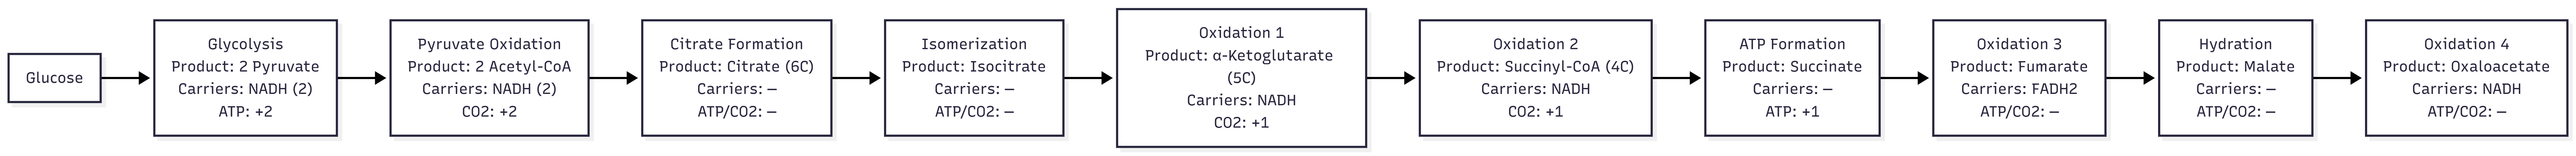
\includegraphics[width=1.05\linewidth]{justins_chart.png}

\vspace{0.5em}
\textit{Justin’s interpretation and chart}
\end{center}
\vspace{1em}

\end{document}